\documentclass[a4j,10pt]{jarticle}

\usepackage[utf8]{inputenc}
\usepackage[japanese]{babel}
\usepackage{minted}

\usepackage[dvipdfmx]{color}
\usepackage[dvipdfmx]{graphicx}
\usepackage{epstopdf}
\usepackage{caption}
\usepackage{subcaption}
\usepackage{cprotect}

\usepackage{import}
\graphicspath{{./img/}}

% 紙面のサイズ
\textwidth=160mm
\textheight=230mm
% マージンの自動調整(紙面の真ん中に配置する)
\setlength{\oddsidemargin}{-2in}
\addtolength{\oddsidemargin}{\paperwidth}
\addtolength{\oddsidemargin}{-\textwidth}
\setlength{\oddsidemargin}{.5\oddsidemargin}
\setlength{\topmargin}{-2in}
\addtolength{\topmargin}{\paperheight}
\addtolength{\topmargin}{-\headheight}
\addtolength{\topmargin}{-\headsep}
\addtolength{\topmargin}{-\topskip}
\addtolength{\topmargin}{-\footskip}
\addtolength{\topmargin}{-\textheight}
\setlength{\topmargin}{.5\topmargin}
% 画像とテキストの占有領域のバランス調整
\renewcommand\textfraction{.2}
%%%%%%%%%%%%%%%%%%%%%%%%%%%%%%%%%%%%%%%%%%%%%%%%%%%%%%%%%%%%%%%%%%%%%%
\title{ %
情報工学実験C% タイトル
\\
{\Large ネットワークプログラミング レポート} % サブタイトル
}
\author{ %
里谷 佳紀 % 氏名
\\
09426568 % 学生番号
}
\date{ %
%出題日: 20xx年xx月xx日\\%
提出日: 2017年1月26日\\%
締切日: 2017年1月26日%
}
%%%%%%%%%%%%%%%%%%%%%%%%%%%%%%%%%%%%%%%%%%%%%%%%%%%%%%%%%%%%%%%%%%%%%%
\begin{document}
\maketitle
%%%%%%%%%%%%%%%%%%%%%%%%%%%%%%%%%%%%%%%%%%%%%%%%%%%%%%%%%%%%%%%%%%%%%%
%\section*{概要}

\section{クライアント・サーバモデルの通信の仕組み}
この章では,クライアント・サーバモデルの通信の一般的な仕組みについて説明する.
クライアントとは,サービスを受けるプログラムやプロセスである.サーバに要求を送り,
受け取った結果を元にさらに処理をする.
サーバとは,サービスを提供するプログラムやプロセスである.クライアントから
要求された処理を行い,その結果をクライアントに送る.
クライアントがサーバと通信するには,プログラムで次の手順を行う必要がある.
\begin{enumerate}
\item サーバの\textbf{IPアドレス}を求める
  (\verb|gethostbyname()|関数で\textbf{ホスト名}から検索することもできる)
\item \verb|socket()|関数で目的の通信形式に合わせて\textbf{ソケット}を作成する
\item \verb|connect()|関数でソケットを元にサーバと通信を開始する
\item \verb|send()|関数でサーバにデータを送信し
  \verb|recv()|関数でサーバからの応答を待つことを繰り返す
\item 通信が終わったら\verb|close()|関数によりソケットを解放する
\end{enumerate}
%各関数を説明する.\verb|gethostbyname()|関数はホスト名を引数にし,
サーバがクライアントと通信するには,次の手順を行う必要がある.
\begin{enumerate}
\item \verb|socket()|関数で目的の通信形式に合わせてソケットを作成する
\item \verb|bind()|関数で作成したソケットに\textbf{ポート番号}などを設定する
\item \verb|listen()|関数で設定したソケットに対するクライアントからの接続要求を待つ
\item \verb|accept()|関数でクライアントからの接続要求を受理して相手先のソケットを
  生成する
\item \verb|recv()|関数でクライアントからのデータを受け付け
  \verb|send()|関数で結果を送信することを繰り返す
\item 通信が終わったら\verb|close()|関数で相手側に接続されたソケットを解放する
\end{enumerate}
%いくつかの関数はクライアント側と共通である.新しく参照した関数を説明する.
クライアント・サーバモデルの通信の手順を図\ref{fig:client-server}にまとめる.
\begin{figure}
  \centering
  %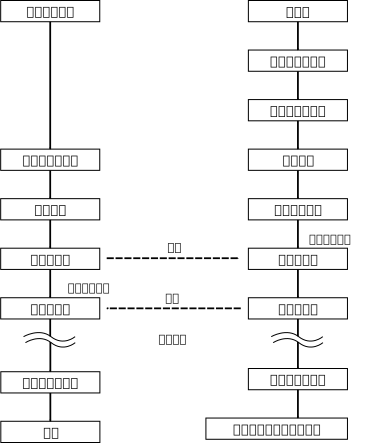
\includegraphics[width=0.5\textwidth]{img/client-server.pdf_tex}
  %\def\svgwidth{\columnwidth}
  \input{img/client-server.pdf_tex}
  \caption{クライアント・サーバモデルの通信の流れ}
  \label{fig:client-server}
\end{figure}
%%%%%%%%%%%%%%%%%%%%%%%%%%%%%%%%%%%%%%%%%%%%%%%%%%%%%%%%%%%%%%%%%%%%%%

\section{プログラムの作成方針}
\label{sec:policy}
本実験では,名簿管理プログラムをクライアント・サーバモデルに対応させる.
この章では開発するプログラムの方針を示し,仕様を与える.
プログラムの方針を以下に挙げる.
\begin{itemize}
\item サーバは名簿データを持つ.さらに,クライアントからの要求を受け,
  名簿データを変形させたり,名簿データを元にクライアントに結果を返す.
\item クライアントは,ユーザからのコマンド入力を元に,サーバに処理の依頼を送る.
  さらにサーバからの結果を処理,表示を行う.
\item プログラミング演習で実装されたコマンドに加え,新たにクライアントからの
  名簿データのアップロードとサーバからの名簿データのダウンロードのコマンドを
  実装する.
\item 通信による遅延を少なくするため,可能な限り通信量を少なくする.
\end{itemize}
以上の方針を考慮して,実装するコマンドの仕様を表\ref{tab:spec-command}に定める.
\begin{table}
  \small
  \centering
  \caption{各コマンドの仕様}
  \label{tab:spec-command}
  \begin{tabular}{lll}
    \hline
    コマンド & 名称 & 処理内容 \\ \hline \hline
    \%C & データチェック &
    \begin{tabular}[t]{ll}
    サーバ & 保持しているデータの概要を送信 \\
    クライアント & サーバからの結果を表示
    \end{tabular} \\ \hline
    \%P \textit{n} & データ表示 &
    \begin{tabular}[t]{ll}
    サーバ & 名簿から指定された件数だけ抜きだし送信 \\
    クライアント & サーバからの結果を表示
    \end{tabular} \\ \hline
    \%R \textit{filename} & 読み込み(サーバ) &
    \begin{tabular}[t]{ll}
    サーバ & 指定されたファイルを読み込み \\
    クライアント & サーバ側の読み込むファイルの名前を送信
    \end{tabular} \\ \hline
    \%RL \textit{filename} & 読み込み(クライアント) &
    \begin{tabular}[t]{ll}
    サーバ & 送信されたデータを保持 \\
    クライアント & クライアントでのファイルを読み込み内容を送信
    \end{tabular} \\ \hline
    \%W \textit{filename} & 書き込み(サーバ) &
    \begin{tabular}[t]{ll}
    サーバ & 保持しているデータをファイルに書き込み \\
    クライアント & サーバでのファイル名をを送信
    \end{tabular} \\ \hline
    \%WL \textit{filename} & 書き込み(クライアント) &
    \begin{tabular}[t]{ll}
    サーバ & 保持しているデータをクライアントに送信 \\
    クライアント & 受信したデータをクライアント側に保存
    \end{tabular} \\ \hline
    \%F \textit{word} & 検索 &
    \begin{tabular}[t]{ll}
    サーバ & \textit{word}に一致するエントリをすべて送信 \\
    クライアント & 受信したデータを表示
    \end{tabular} \\ \hline
    \%S \textit{col} & ソート &
    \begin{tabular}[t]{ll}
    サーバ & 列番号\textit{col}を基準にした並べ替えを実行 \\
    クライアント & 列番号\textit{col}をサーバに送信
    \end{tabular} \\ \hline
    \%Q & 終了 &
    \begin{tabular}[t]{ll}
    サーバ & クライアントとの接続を遮断 \\
    クライアント & サーバに通信終了の旨を送信しプログラムを終了
    \end{tabular} \\ \hline
  \end{tabular}
\end{table}
%%%%%%%%%%%%%%%%%%%%%%%%%%%%%%%%%%%%%%%%%%%%%%%%%%%%%%%%%%%%%%%%%%%%%%

\section{プログラムの実装}
\subsection{データ構造とデータの流れ}
開発したプログラムの実装を説明する.まず,実装に使用したデータ構造を説明する.
名簿のデータはサーバがファイルから読み込むか,クライアントからアップロードされる
ことでサーバに保持される.そのため,サーバプログラムの\verb|server.c|には,
一件の名簿のデータ\verb|profile|構造体の配列の\verb|current_profile_table|
グローバル変数と,\verb|profile|構造体のポインタの配列\verb|current_profile_view|
グローバル変数を持つ.\verb|profile|構造体の内容を
表\ref{tab:definition-of-profile}に示す.
\begin{table}
  \centering
  \cprotect\caption{\verb|profile|構造体の定義}
  \label{tab:definition-of-profile}
  \begin{tabular}{crl}
    \hline
    メンバ名 & 大きさ(byte) & 説明 \\ \hline \hline
    \verb|id| & 4 & 識別番号 \\ \hline
    \verb|name| & 70 & 名前(文字配列) \\ \hline
    \verb|est| & 6 & 日付(年,月,日それぞれ2byte) \\ \hline
    \verb|addr| & 70 & 所在地(文字配列) \\ \hline
    \verb|misc| & 任意 & 説明(文字配列へのポインタ) \\ \hline
  \end{tabular}
\end{table}
サーバは,クライアントからサーバにあるファイルの読み込み要求や,クライアント
からのデータのアップロードがあると,データの実体を\verb|current_profile_table|に
格納し,\verb|current_profile_table|の一件ごとの参照を並べて
\verb|current_profile_view|とする.
また,クライアントから整列の要求が来ると,名前などの基準に応じて
\verb|current_profile_view|の参照を入れ替える.このとき,
\verb|current_profile_table|に対する操作はない.
さらに,クライアントから探索や表示の要求が来ると,\verb|current_profile_view|から
該当するデータを抜きだし,クライアントに返す.
\verb|current_profile_table|の内容は,次にサーバがファイルを読むか,
クライアントから名簿データを受信すると上書きされる.
サーバ上にある\verb|current_profile_table|と\verb|current_profile_view|,
サーバ上にある名簿データを格納したファイルとクライアントの関係を
図\ref{fig:table-and-view}にまとめる.
\begin{figure}
  \centering
  \def\svgwidth{\columnwidth}
  \input{img/system.pdf_tex}
  \caption{システムの概要図 \\ \footnotesize{
      クライアントの,サーバのファイルに対する読み込み要求と書き込み要求を
      省略している.}}
  \label{fig:table-and-view}
\end{figure}
\subsection{処理の流れと通信プロトコル}
処理の流れと使用する通信プロトコルをクライアント側とサーバ側に分けて説明する.
クライアントが送るデータとサーバが送るデータの様子を図\ref{fig:basic-data}に示す.
クライアントプログラムが送信するデータは次の要素を含む.
\begin{itemize}
\item 送信するデータの大きさ(4byte)
\item サーバに実行を要求するコマンドの種類(2byte)
\item コマンドごとに異なるデータ(任意の長さ)
\end{itemize}
これらを,データの大きさとそれ以外の2回に分けて送信する.こうすることで,サーバ
プログラムが読み取るべきデータの大きさを認識できる.
コマンドの種類は\verb|common.h|の\verb|command_index|型として定義される.
サーバプログラムが送信するデータは次の要素を含む.
\begin{itemize}
\item 送信するデータの大きさ(4byte)
\item サーバが実行したコマンドの種類(2byte)
\item ステータスコード(2byte)
\item コマンドごとに異なるデータ(任意の長さ)
\end{itemize}
これらを,クライアントと同様に2回に分けて送信する.
実行したコマンドの種類を送る理由は,サーバが要求通りのコマンドを実行したかを
クライアントでチェックできるようにするためである.
ステータスコードとは,要求されたコマンドが正しく実行できたか,あるいは何らかの
エラーが発生したかを示す.例えば,ソートコマンドで範囲外の列番号が指定された場合,
サーバは\verb|profile.h|の\verb|PS_INVCOL|をステータスコードとしてクライアントに
送る.
\begin{figure}
  \centering
  \subcaptionbox{
    クライアントが送信するデータ\label{fig:client-data}}{
    \input{img/client-data.pdf_tex}}
  \par\bigskip
  \subcaptionbox{
    サーバが送信するデータ\label{fig:server-data}}{
    \input{img/server-data.pdf_tex}}
  \caption{コマンドに共通するデータ(数字はbyte単位)}
  \label{fig:basic-data}
\end{figure}

コマンドごとに異なるデータの内容を表\ref{tab:command-and-data}に示す.
\begin{table}
  \footnotesize
  \centering
  \caption{各コマンドで送信されるデータ}
  \label{tab:command-and-data}
  \begin{tabular}{llll}
    \hline
    コマンド & クライアントが送信するデータ & サーバが送信するデータ &
    ステータスコード \\
    \hline \hline
    \%C & なし & 保持しているデータの件数(4byte) &
    \begin{tabular}[t]{l}
      常に\verb|PS_SUCCESS|
    \end{tabular} \\ \hline
    \%P & 表示するデータの件数(4byte) & 要求された件数を持つ\verb|profile_table| &
    \begin{tabular}[t]{l}
      \textit{n}が0の場合\verb|PS_INVARG| \\ それ以外は\verb|PS_SUCCESS|
    \end{tabular} \\ \hline
    \%R & ファイル名(4byte+1byte$\times$長さ) & 読み取った件数(4byte) &
    \begin{tabular}[t]{l}
      常に\verb|PS_SUCCESS| \\ (エラーチェック未実装)
    \end{tabular} \\ \hline
    \%RL & 読み取った件数を持つ\verb|profile_table| & 読み取った件数(4byte) &
    \begin{tabular}[t]{l}
      常に\verb|PS_SUCCESS| \\ (エラーはクライアント側で検知)
    \end{tabular} \\ \hline
    \%W & ファイル名(4byte+1byte$\times$長さ) & 書き込んだ件数(4byte) &
    \begin{tabular}[t]{l}
      常に\verb|PS_SUCCESS| \\ (エラーチェック未実装)
    \end{tabular} \\ \hline
    \%WL & なし & 保持している\verb|profile_table| &
    \begin{tabular}[t]{l}
      常に\verb|PS_SUCCESS|
    \end{tabular} \\ \hline
    \%F & 検索語(4byte+1byte$\times$長さ) & 検索結果の\verb|profile_table| &
    \begin{tabular}[t]{l}
      常に\verb|PS_SUCCESS| \\ (エラーはクライアント側で検知)
    \end{tabular} \\ \hline
    \%S & 基準となる列(2byte) & なし &
    \begin{tabular}[t]{l}
      有効な列番号は\verb|PS_SUCCESS| \\ それ以外は\verb|PS_INVCOL|
    \end{tabular} \\ \hline
    \%Q & なし & なし &
    \begin{tabular}[t]{l} 常に\verb|PS_SUCCESS| \end{tabular}
    \\ \hline
  \end{tabular}
\end{table}
表中にある\verb|profile_table|構造体は,\verb|profile.h|で定義される.
\verb|profile_table|構造体は,\verb|profile|構造体の配列と格納する\verb|profile|
構造体の数を格納する.\verb|profile_table|構造体を送信するには,次の要領で
整列化する(\verb|profile.c|の\verb|serialize_profile_table|,
\verb|serialize_profile_view|参照).
\begin{enumerate}
\item 格納する\verb|profile|構造体の数\verb|n_entries|を整列化する.
\item \verb|entries|メンバの要素を順に\verb|n_entries|個だけ整列化する.
  表\ref{tab:definition-of-profile}を参考に整列化する.
  \begin{enumerate}
  \item \verb|id|メンバを整列化する.バイトオーダを揃える\verb|htonl|関数を用いる.
  \item \verb|name|メンバを整列化する.英数字を扱っているため,今回はバイトオーダを
    考慮する必要はない.
  \item \verb|est|メンバを整列化する.\verb|date|構造体の整列化であるが2byteの
    整数型のメンバが3つ集まったものと解釈してよい.
  \item \verb|addr|メンバを整列化する.
  \item \verb|misc|メンバの長さを整列化する(4byte).
  \item \verb|misc|メンバの実体を整列化する.
  \end{enumerate}
\end{enumerate}
%%%%%%%%%%%%%%%%%%%%%%%%%%%%%%%%%%%%%%%%%%%%%%%%%%%%%%%%%%%%%%%%%%%%%%

\section{プログラムの使用法}
\label{sec:usage}
プログラムの使用法を例に沿って説明する.クライアントプログラム\verb|client.out|と
テスト用のデータ\verb|sample.csv|が\verb|~MyDirectory|に,
サーバプログラム\verb|server.out|が\verb|~YourDirectory|にあると仮定する.
まず,\verb|server.out|をポート番号を与えて実行する.例えば,
\begin{verbatim}
./server.out 9000
\end{verbatim}
とする.プログラムが起動すると,クライアントの接続を待つ.次にサーバ側のホスト名と
ポート番号を与えて\verb|client.out|を起動する.例えば.
\begin{verbatim}
./client.out localhost 9000
\end{verbatim}
とする.起動後,サーバと接続に成功するとコマンド入力が促される.

以後,実行例としてファイルのアップロードと編集,サーバ側への書き込みを示す.
まず,クライアント側で\verb|%RL|コマンドを使って\verb|sample.csv|の内容を
サーバへ送信する.具体的には,
\begin{verbatim}
%RL sample.csv
\end{verbatim}
とする.実行後,ファイルの内容がサーバにアップロードされる.次に,確認のため,
\verb|%C|コマンドで読み込んだ名簿の件数を確認し,\verb|%P|コマンドで最初の1件
を表示する.
\begin{verbatim}
%C
\end{verbatim}
を実行すると,
\begin{verbatim}
2886 profiles in view
\end{verbatim}
と表示される.また,
\begin{verbatim}
%P 1
\end{verbatim}
を実行すると,
\begin{verbatim}
ID:	5100046
Name:	The Bridge
Est.:	1845/11/2
Addr.:	14 Seafield Road Longman Inverness
Misc.:	SEN Unit 2.0 Open

\end{verbatim}
と表示される.さらに,\verb|%S|コマンドでこのデータを名前順に並べ替える.
\begin{verbatim}
%S 2
\end{verbatim}
を実行すると,並び替えが終了した旨のメッセージが返ってくる.
ここで\verb|%P|コマンドで最初の1件を表示すると,
\begin{verbatim}
ID:	8212627
Name:	Abbey Primary School
Est.:	1918/8/23
Addr.:	Claremont Crescent Kilwinning
Misc.:	01294 552251 01294 550525 Primary 295 10.5 Open

\end{verbatim}
と表示される.

最後に,このデータをサーバ側のファイルに書き込む.\verb|%W|コマンドを
\begin{verbatim}
%W sample2.csv
\end{verbatim}
として実行すると,\verb|server.out|がある\verb|~/YourDirectory|に\verb|sample2.csv|が
保存される.\verb|%Q|コマンドで終了して,\verb|sample2.csv|の内容を確認すると,
\begin{verbatim}
8212627,Abbey Primary School,...
5520924,Abbeyhill Primary School,...
5237521,Abbotswell School,...
\end{verbatim}
となっており,名前順で並び替えしたのちに保存できたことが分かる.
%%%%%%%%%%%%%%%%%%%%%%%%%%%%%%%%%%%%%%%%%%%%%%%%%%%%%%%%%%%%%%%%%%%%%%

\section{プログラムの作成過程に関する考察}
\subsection{工夫した点}
主に工夫した点は,整列化と非整列化である.これにより,文字列だけを送受信する
場合に比べて扱えるデータの種類が増え,やりとりするデータ量が小さくなることが
期待できる.データ量の改善については,\ref{sec:concl}で考察する.

また,ネットワークプログラムとは直接関係ないが,名簿のエントリの参照を並べる
データ構造\verb|profile_view|を採用することで,更なる機能を追加できる.
例えば,クライアントがサーバに現在のデータから新しく\verb|profile_view|を
作成する要求を出せるようにする機能などが考えられる.

\subsection{苦労した点}
苦労した点もやはり整列化と非整列化である.非整列化のときに,プロトコルで定義した
データの大きさを超えるデータを受信することによる不具合があった.
緊急の処置として,プロトコルで定義したデータの大きさだけ受信したら,
次の要求までのデータを無効化することを行った.具体的には,
\verb|select()|関数を使って\verb|recv()|にタイムアウトを設けつつ,\verb|recv()|で
受信データを読み込み続けることを繰り返した.原因は今でも分かっていないので,
今後の課題の一つである.
%%%%%%%%%%%%%%%%%%%%%%%%%%%%%%%%%%%%%%%%%%%%%%%%%%%%%%%%%%%%%%%%%%%%%%

\section{得られた結果に関する考察}
\label{sec:concl}
ここで,開発したプログラムが\ref{sec:policy}の方針を満足するか振り返る.
\ref{sec:policy}で示した方針を再び示す.
\begin{itemize}
\item\label{item:req:srv} サーバは名簿データを持つ.さらに,クライアントからの
  要求を受け,名簿データを変形させたり,名簿データを元にクライアントに結果を返す.
\item\label{item:req:cln} クライアントは,ユーザからのコマンド入力を元に,
  サーバに処理の依頼を送る.さらにサーバからの結果を処理,表示を行う.
\item\label{item:req:cmd} プログラミング演習で実装されたコマンドに加え,
  新たにクライアントからの名簿データのアップロードとサーバからの名簿データの
  ダウンロードのコマンドを実装する.
\item\label{item:req:cmn} 通信による遅延を少なくするため,
  可能な限り通信量を少なくする.
\end{itemize}
4つの方針のうち,上の三つは,\ref{sec:usage}に実例を示したとおり,達成できた.
最後の方針について考察する.\verb|sample.csv|を対象に,
ファイルをそのまま文字列で送信した場合と,整列化して送信した場合とを比較する.
まず,ファイルをそのまま送信する場合のデータ量は,Linuxの
\verb|wc|コマンドで見ることができ,343021byteである.
整列化して送信する場合のデータ量を計算する.表\ref{tab:definition-of-profile}
より,1件の名簿の固定長の部分の大きさは,$4+70+6+70+4=154$byteである.
残りの領域は,\verb|misc|メンバが指す先の長さである.\verb|sample.csv|は,
Linuxで\verb^awk -F "\"*,\"*" '{print $5}' sample.csv | wc^で計算する.
全体で143052byteであるが,2885個の改行が含まれ,整列化はヌル文字を含むので,
実際の大きさは$143052-2885+2886=143053$byteである.以上のことから,
整列化して送信する場合のデータ量は,送信する名簿の件数4byteを足して,
$4+154\times 2886+143053=587501$byteである.これは,ファイルをそのまま送る方法
に比べて大きく,方針は達成できなかった.原因は,\verb|name|メンバと\verb|addr|メンバ
が無駄に大きな領域をとっていることがある.また,送信するデータのほとんどが文字列で,
整列化によるデータ量削減の効果が薄くなることも原因と考えられる.
%%%%%%%%%%%%%%%%%%%%%%%%%%%%%%%%%%%%%%%%%%%%%%%%%%%%%%%%%%%%%%%%%%%%%%
\newpage

\appendix
\section{プログラムリスト}
\subsection{client.c}
\inputminted[linenos,fontsize=\footnotesize]{C}{../src/client.c}
\subsection{server.c}
\inputminted[linenos,fontsize=\footnotesize]{C}{../src/server.c}
\subsection{common.h}
\inputminted[linenos,fontsize=\footnotesize]{C}{../src/common.h}
\subsection{profile.h}
\inputminted[linenos,fontsize=\footnotesize]{C}{../src/profile.h}
\subsection{profile.c}
\inputminted[linenos,fontsize=\footnotesize]{C}{../src/profile.c}
\subsection{date.c}
\inputminted[linenos,fontsize=\footnotesize]{C}{../src/date.c}
\subsection{buffer.c}
\inputminted[linenos,fontsize=\footnotesize]{C}{../src/buffer.c}
\subsection{mystring.c}
\inputminted[linenos,fontsize=\footnotesize]{C}{../src/mystring.c}


%%%%%%%%%%%%%%%%%%%%%%%%%%%%%%%%%%%%%%%%%%%%%%%%%%%%%%%%%%%%%%%%%%%%%%
\end{document}
